\chapter{Model Structure}

In the previous chapter, we introduced the foundational algorithms employed in this research project. This chapter delves into the structure of our custom Transformer-based model, designed to predict the "score" or gradient in detector simulations. Built upon the Transformer architecture—a cutting-edge model in deep learning—our model incorporates several modifications to enhance its applicability in high-energy physics detector simulations.

We chose the Transformer architecture not only for its power and versatility but also for its unique suitability for data with rotational invariance. In our research, each input consists of multiple showers, each shower containing several hits, and each hit represented by four features, as introduced in Chapter 3. This structure makes our data rotationally invariant, meaning that the relationships within the data remain consistent even if the order of hits within a shower or the showers within an input are rearranged. Transformers are particularly well-suited for handling such properties. Their self-attention mechanism enables them to learn and capture relationships between data points in a way that is invariant to transformations like rotation. This flexibility is especially advantageous for our detector simulations, where capturing invariant relationships is crucial for making accurate predictions.

We will begin by exploring the evolution of Transformers from Recurrent Neural Networks (RNNs), highlighting how Transformer architectures overcame the limitations of sequential models. Following this, we will examine the core components of the Transformer model, including its different architectural types (encoder-only, decoder-only, and encoder-decoder models) and the self-attention mechanism, which lies at the heart of the Transformer’s ability to model long-range dependencies.

After establishing an understanding of the original Transformer architecture, we will discuss the custom modifications introduced in our model to optimize it for detector simulations. Key innovations include the \textbf{Gaussian Fourier Projection} for encoding temporal information, which allows the model to capture high-frequency dependencies by transforming time and incident energy into sinusoidal features. Additionally, we introduce a specialized \textbf{mean-field attention mechanism}, a variant of self-attention tailored to efficiently aggregate global context. Mean-field attention leverages a class token to summarize information across the sequence, reducing computational complexity while retaining essential global information.

Furthermore, our model incorporates residual network structures and layer normalization to stabilize and expedite the training process. We will explain how these modifications, along with our encoder-only architecture, facilitate efficient information flow, enabling the model to focus on capturing the relationships within the data rather than generating sequences. We also employ \textbf{Weights \& Biases (wandb)} for parameter tuning, using its sweep functionality to systematically explore hyperparameters such as the number of encoder blocks, attention heads, and dropout rates to achieve optimal performance.

In summary, this chapter provides a comprehensive overview of our custom Transformer model, from its foundational components to the innovative adjustments that make it well-suited for high-energy physics applications. Through these design choices, our model efficiently captures both local and global dependencies, thereby enhancing the accuracy and fidelity of detector simulations.

\section{Transformer}

\subsection{Introduction}
Transformer models have transformed deep learning applications across various domains, providing significant advantages in handling complex and large datasets. In high-energy physics, where data from detectors is vast and multidimensional, advanced models like Transformers enhance both the accuracy and efficiency of simulations designed to emulate particle collisions and energy depositions within detectors.

\subsection{The Evolution from RNNs to Transformers}
Prior to Transformers, Recurrent Neural Networks (RNNs) were widely used for sequence modeling due to their ability to capture dependencies between sequential elements. However, RNNs are inherently sequential, making them slow and prone to issues like vanishing gradients, particularly with long sequences.

The introduction of Transformers by Vaswani et al. in their seminal paper, \textit{"Attention is All You Need,"} addressed these limitations by introducing the self-attention mechanism. This innovation enables Transformers to capture long-range dependencies without the need for recurrent connections, allowing for faster and more efficient training.

\begin{figure}[ht]
    \centering
    \begin{subfigure}[b]{0.45\textwidth}
        \centering
        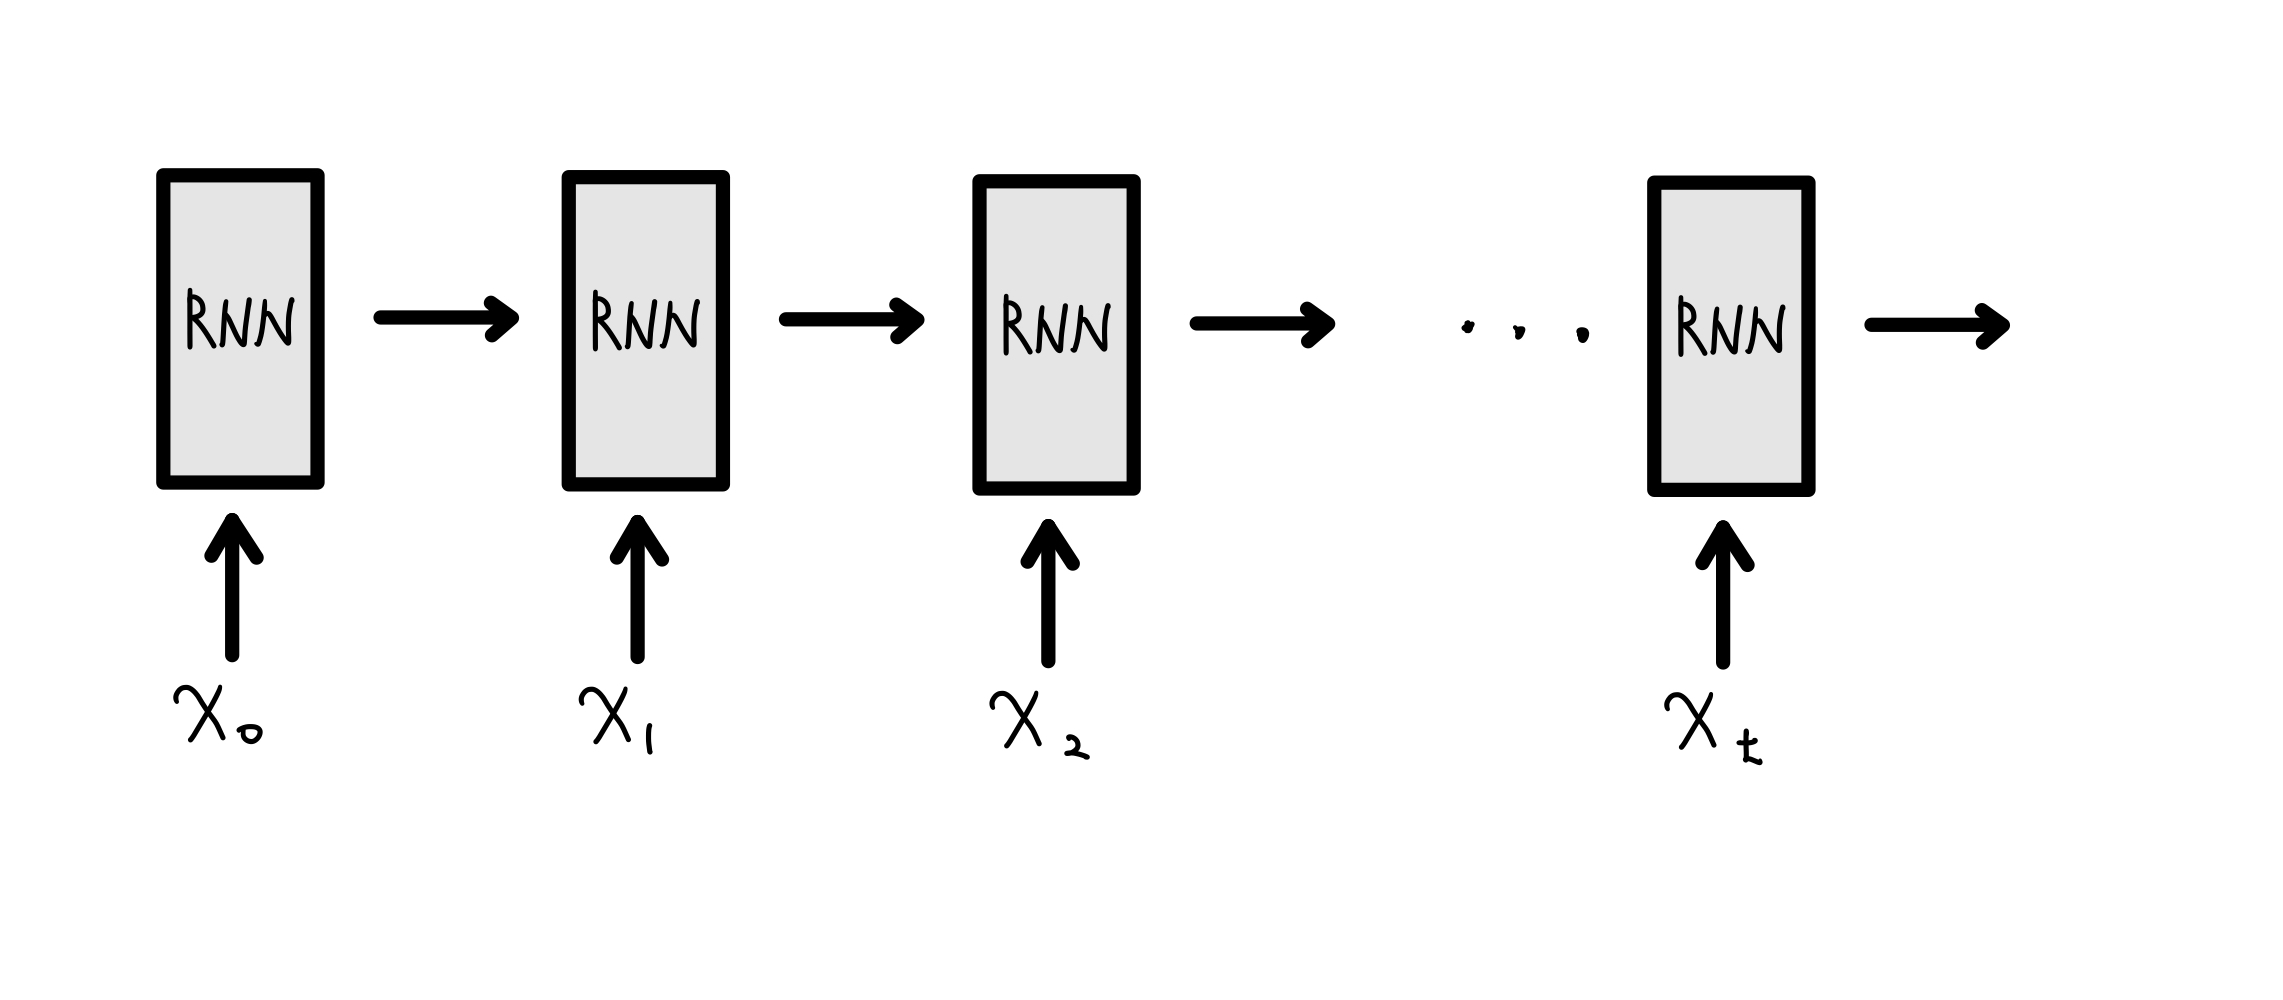
\includegraphics[width=\textwidth]{Figures/rnn.jpeg}
        \caption{RNN Model}
        \label{fig:rnn}
    \end{subfigure}
    \hfill
    \begin{subfigure}[b]{0.45\textwidth}
        \centering
        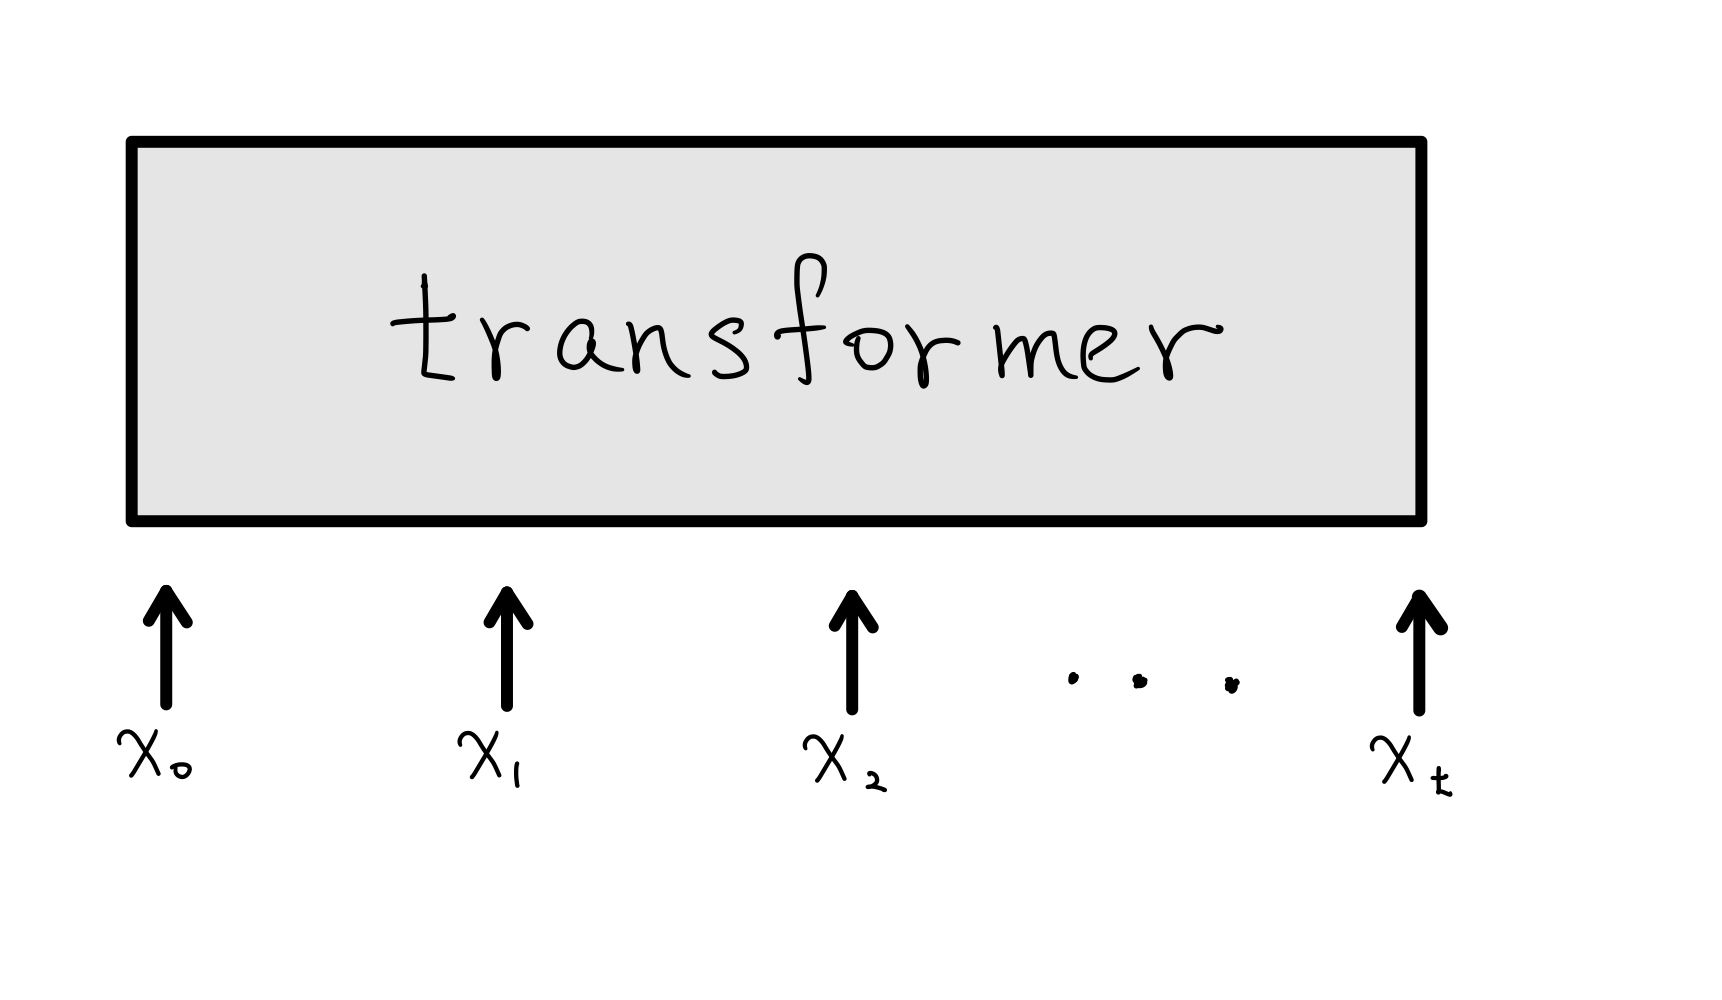
\includegraphics[width=\textwidth]{Figures/transformer.jpeg}
        \caption{Transformer Model}
        \label{fig:transformer}
    \end{subfigure}
    \caption{Comparison of RNN and Transformer architectures.}
    \label{fig:comparison}
\end{figure}

\subsection{Types and Structure of Transformer Architectures}
The original Transformer architecture, as introduced by Vaswani et al., consists of both an encoder and a decoder. The encoder processes the input sequence, while the decoder generates the output sequence. This setup is particularly effective for tasks like machine translation. However, in practice, different applications benefit from using only the encoder or decoder.

\begin{figure}[ht]
    \centering
    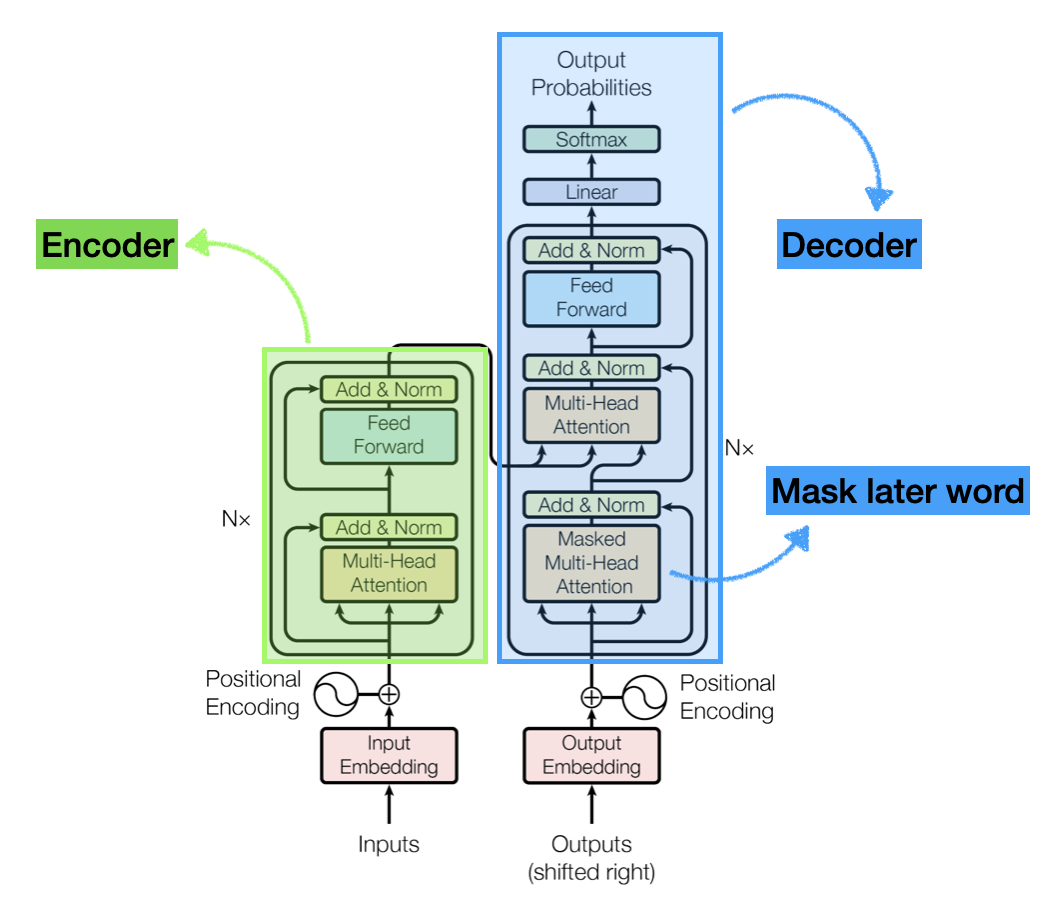
\includegraphics[width=0.8\textwidth]{Figures/transformerblock.png}
    \caption{The structure of the original Transformer model. Adapted from \textit{"Attention is All You Need,"} with additional annotations.}
    \label{fig:transformer_structure}
\end{figure}

The three main types of Transformer architectures are as follows:

\begin{itemize}
    \item \textbf{Encoder-only Models}: Encoder-only models, such as BERT, create contextual embeddings by attending to all tokens bidirectionally. These models are ideal for tasks requiring sequence understanding, like classification.
    
    \item \textbf{Decoder-only Models}: Decoder-only models, like GPT, are designed for unidirectional generation. Each token attends only to previous tokens, making these models suitable for tasks like language modeling.
    
    \item \textbf{Encoder-Decoder Models}: The original Transformer model combines both an encoder and a decoder, making it effective for sequence-to-sequence tasks such as machine translation. Examples include BART and T5.
\end{itemize}

\subsection{Choosing an Encoder-Only Model for Detector Simulation}
In the context of detector simulation, our objective is to generate a high-quality representation of input data, such as particle collisions, without generating new sequences. Thus, an encoder-only model is more appropriate, as it efficiently processes and encodes input data, capturing necessary features without the additional complexity of a generative decoder.

\section{Self-Attention Mechanism}
Self-attention is central to the Transformer model, enabling each token in a sequence to attend to all other tokens. For each token, the attention scores are computed based on the query \( Q \), key \( K \), and value \( V \) vectors:

\begin{equation}
\text{Attention}(Q, K, V) = \text{softmax} \left( \frac{QK^T}{\sqrt{d_k}} \right) V
\end{equation}

This mechanism allows the model to capture relationships between distant tokens, which is crucial for high-dimensional data, such as particle detector simulations. Figure ?? illustrates the self-attention mechanism, showcasing how each token dynamically weights other tokens in the sequence.

\section{Our Model Structure}
Our model architecture builds upon the Transformer framework, with specific modifications to optimize performance in detector simulations, as shown in Figure .

\begin{figure}[ht]
    \centering
    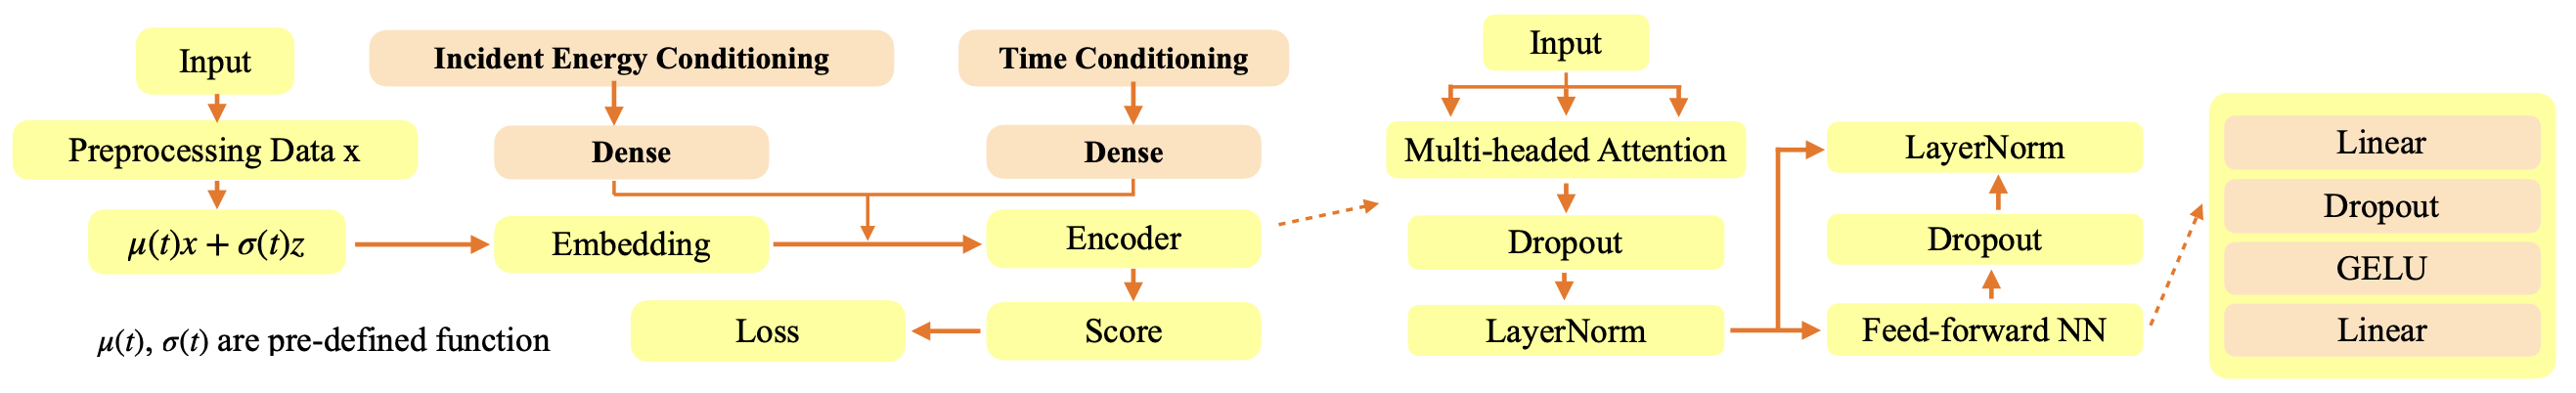
\includegraphics[width=0.8\textwidth]{Figures/model_structure.png}
    \caption{Custom Transformer model structure for detector simulations.}
    \label{fig:model_structure}

\end{figure}
We incorporate \textbf{Gaussian Fourier Projections} \cite{tancik_fourier_2020} to effectively encode temporal information, dense layers to transform conditional variables, and \textbf{mean-field attention} \cite{kach_pay_2024} to efficiently aggregate global context. These architectural choices enable our model to capture complex dependencies, thereby enhancing the fidelity and accuracy of simulation outcomes.

\subsection{Gaussian Fourier Projection for Temporal Encoding}
The Gaussian Fourier Projection component encodes temporal information using Gaussian random features. This technique allows the model to incorporate high-frequency time-dependent information, in our case time and incident energy, which is crucial for capturing the dynamics of particle interactions within detectors.

In our model, we apply a Fourier feature mapping \( \gamma \) to featurize input coordinates before passing them through a coordinate-based multilayer perceptron (MLP). This approach improves both convergence speed and generalization.

The mapping function \( \gamma \) transforms input points \( \mathbf{v} \in [0, 1)^d \) onto the surface of a higher-dimensional hypersphere using sinusoidal functions:

\begin{equation}
\gamma(\mathbf{v}) = 
\begin{bmatrix}
a_1 \cos(2 \pi \mathbf{b}_1^T \mathbf{v}) \\ 
a_1 \sin(2 \pi \mathbf{b}_1^T \mathbf{v}) \\ 
\vdots \\ 
a_m \cos(2 \pi \mathbf{b}_m^T \mathbf{v}) \\ 
a_m \sin(2 \pi \mathbf{b}_m^T \mathbf{v})
\end{bmatrix}
\end{equation}

where \( a_i \) and \( \mathbf{b}_i \) are parameters that control the scaling and frequency of each sinusoid. We set \( a = 1 \) for all cases and experiment with different values of \( \mathbf{b} \) to identify optimal performance. The results are presented in subsequent sections.

\subsection{Mean-Field Attention in Detector Simulation}
Our model utilizes a variation of self-attention called \textbf{mean-field attention}. Unlike traditional self-attention, mean-field attention employs a class token to aggregate information from all tokens, creating a global summary. This reduces computational complexity while preserving essential global context.

Mean-field attention allows the class token to encapsulate the sequence's essential features by attending to each token once. This mechanism is computationally efficient and well-suited for high-energy physics applications, where capturing global properties of particle collisions is more important than individual token interactions. Figure ?? provides a comparison between self-attention and mean-field attention mechanisms.

\begin{figure}[ht]
    \centering
    \begin{subfigure}[b]{0.35\textwidth}
        \centering
        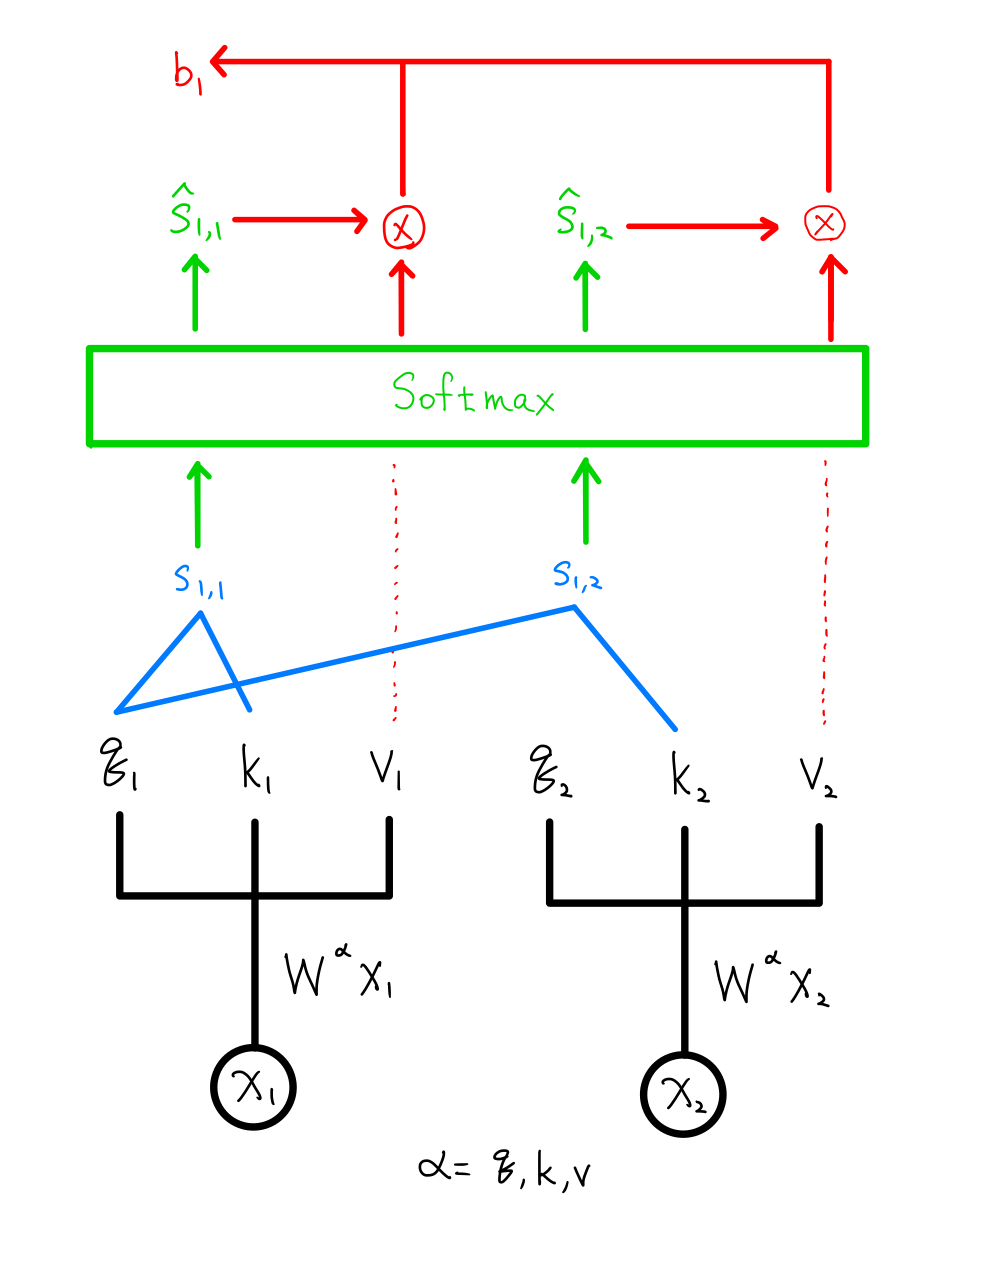
\includegraphics[width=\textwidth]{Figures/selfattention.jpeg}
        \caption{Self-Attention Mechanism}
        \label{fig:self_attention}
    \end{subfigure}
    \hfill
    \begin{subfigure}[b]{0.45\textwidth}
        \centering
        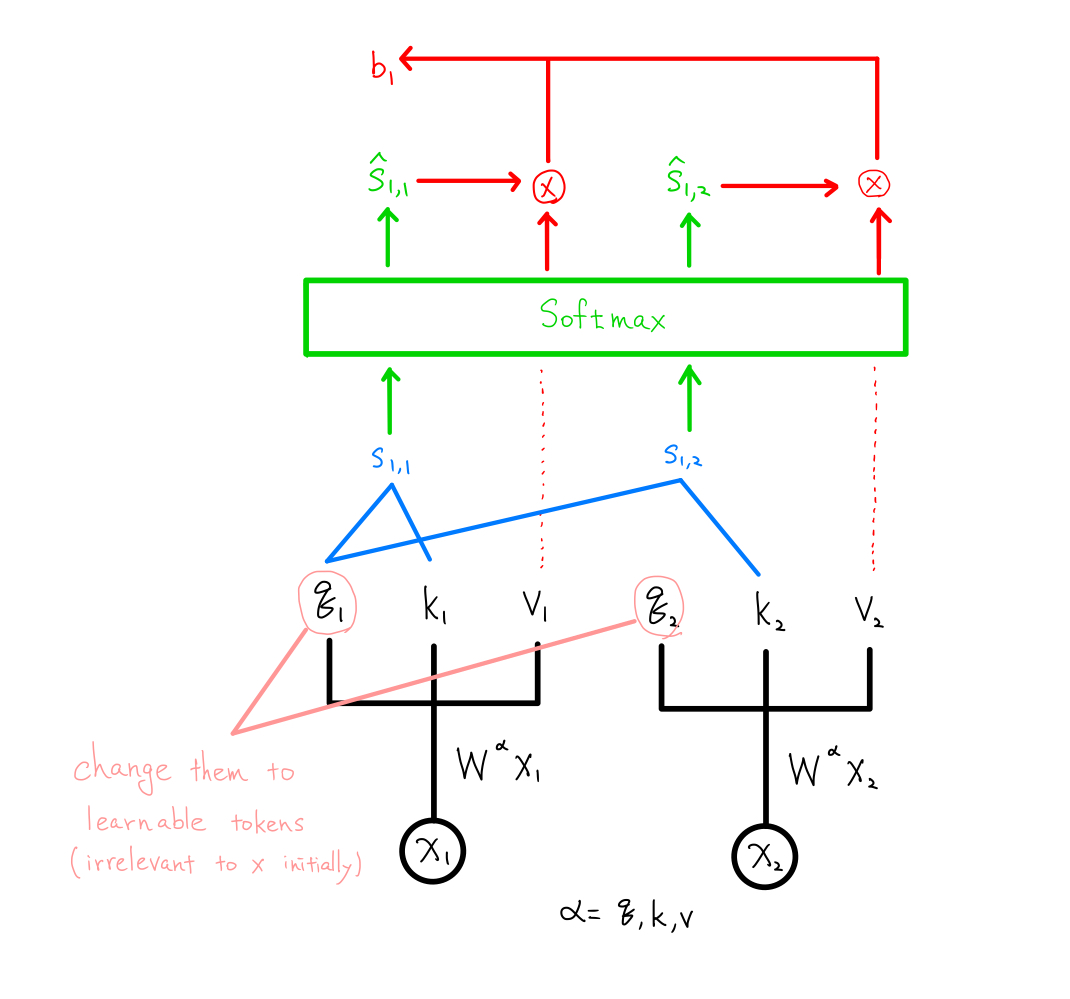
\includegraphics[width=\textwidth]{Figures/meanfield.jpeg}
        \caption{Mean-Field Attention Mechanism}
        \label{fig:mean_field_attention}
    \end{subfigure}
    \caption{Comparison of self-attention and mean-field attention mechanisms.}
    \label{fig:attention_comparison}
\end{figure}

\subsection{Parameter Tuning}
Once the model structure is established, tuning the parameters is essential for optimal performance. 

To optimize the model, we utilize \textbf{Weights \& Biases (wandb)} for parameter tuning. Using wandb’s sweep functionality, we systematically explore hyperparameters, including:

\begin{itemize}
    \item \textbf{Number of blocks}: Controls the depth of the Transformer model.
    \item \textbf{Number of heads}: Determines the number of attention heads in the multi-head attention mechanism.
    \item \textbf{Hidden dimension}: Sets the size of the hidden layers in the model.
    \item \textbf{Embed dimension}: Specifies the embedding size for the model’s input.
    \item \textbf{Batch size}: Number of samples per batch.
    \item \textbf{Learning rate}: Determines the rate at which the model updates during training.
    \item \textbf{Dropout rate}: The fraction of nodes dropped during training to prevent overfitting.
    \item \textbf{Sampling steps}: The number of sampling steps when solving SDE.
    \item \textbf{Correction steps}: The number of correction steps in each sampling step.
    \item \textbf{Scale in Fourier features}: The scaling factor for Fourier features.
\end{itemize}

The results of this tuning process are presented in later chapters.

\section{Conclusion}
Our custom Transformer model leverages specialized architectural choices to optimize performance in high-energy physics simulations. Key modifications include \textbf{Gaussian Fourier projections} for encoding time and incident energy, and \textbf{mean-field attention} for capturing global context beyond immediate shower information. The addition of a class token enables the model to represent both local and global dependencies, making it particularly suitable for scenarios with strong temporal and energetic relationships.

The mean-field attention mechanism enhances computational efficiency by reducing complexity while preserving essential global information. Parameter tuning plays a crucial role in achieving optimal performance, as we demonstrate with our use of wandb. By employing an encoder-only model, we capture inter-token relationships within the data, making our approach well-suited for high-energy physics applications.
